\documentclass{article}
\usepackage[T2A]{fontenc}
\usepackage[utf8]{inputenc}
\usepackage[russian]{babel}
\usepackage{amssymb,amsmath,amsthm}
\usepackage{systeme,mathtools}
\usepackage{lipsum}
\usepackage{relsize}
\newcommand\md{\ }
\usepackage[normalem]{ulem}
\usepackage{pdfpages}

\begin{document}
\selectlanguage{russian}

\includepdf[pages=-]{Ok.pdf}
\section{Задание}

1.Прочитать UML диаграмму: на диаграмме представлены Абстрактный суперкласс Shape и его подклассы Circle, Rectangle и Square.
2.Перепишите суперкласс Shape и его подклассы так как это представлено на UML диаграмме Circle, Rectangle and Squar

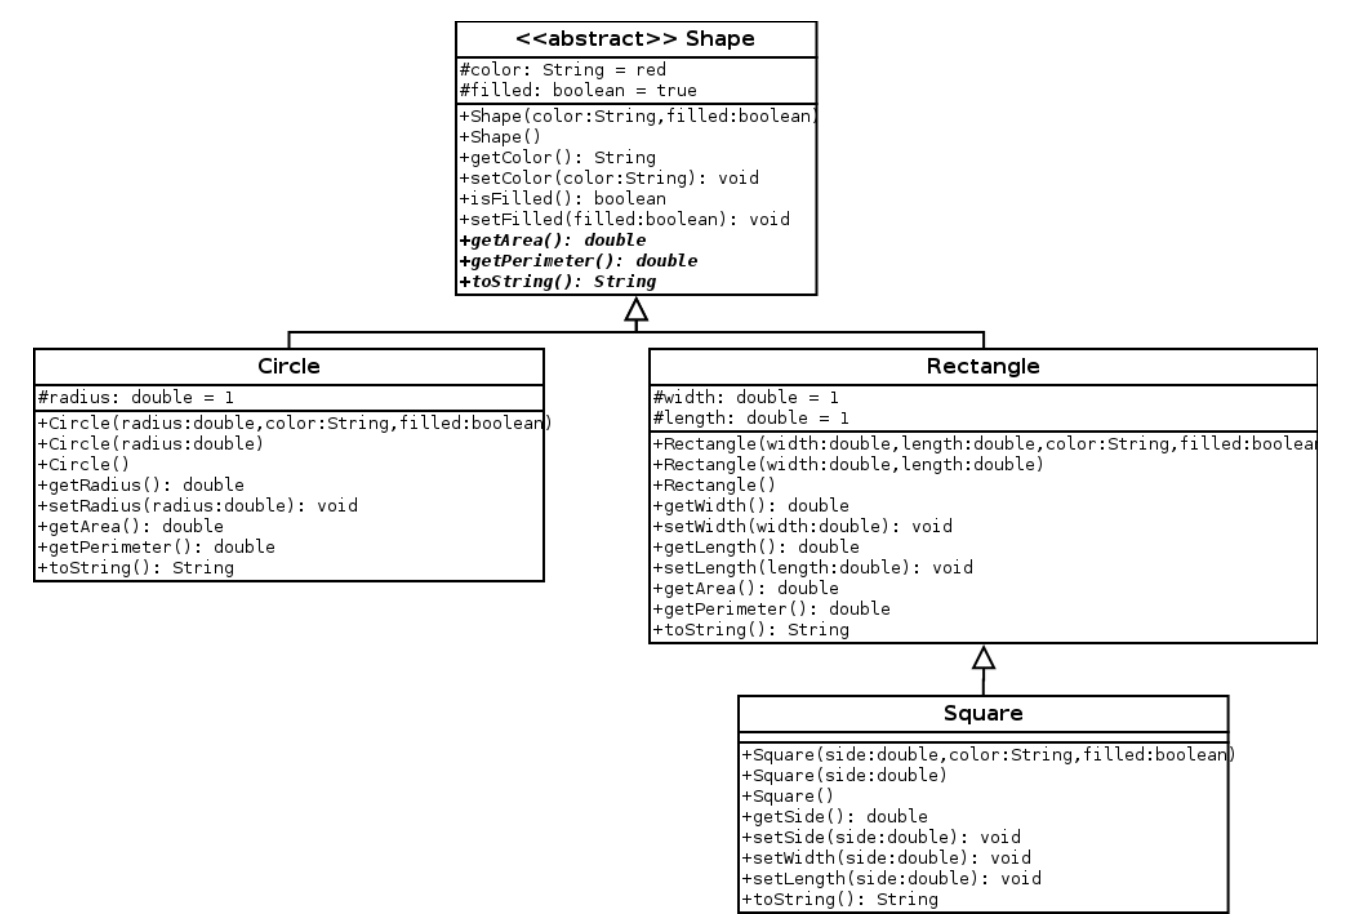
\includegraphics[width=1\linewidth]{pic.jpg}

\caption{Рисунок 1. UML диаграмма.}

\section{Ход работы}

В ходе выполнения работы были получены следующий исходный код:
\begin{verbatim}
package com.company;
import java.lang.Math.*;

public class Main {
    public static void main(String[] args) {
        Circle OneCircle = new Circle(7,"Coral",true); //If False, OUTPUT: " "
        Rectangle OneRectangle = new Rectangle(6,5,"Azure",true);
        Square NewSquare = new Square(7,"Maroon",true);

        System.out.print(OneCircle.toString()+"\n" + OneRectangle.toString() 
                                                   + "\n" + NewSquare.toString());
    }
}

abstract class Shape {
    protected String Colour = "red";
    protected boolean Filled = true;

    public Shape(String Colour, boolean Filled){
        this.Colour = Colour;
        this.Filled = Filled;
    }

    public Shape(){}

    public void setColour(){ this.Colour = Colour; }
    public void setFilled(){ this.Filled = Filled; }
    public String getColour(){ return Colour; }
    public boolean isFilled(){ return Filled; }
}

class Rectangle extends Shape{
    double Width = 1;
    double Length = 1;

    public Rectangle(double Width, double Length, String Colour, boolean Filled){
        this.Width = Width;
        this.Length = Length;
        this.Colour = Colour;
        this.Filled = Filled;
    }

    public Rectangle(double Width, double Length){
        this.Width = Width;
        this.Length = Length;
    }

    public Rectangle(){}

    public double getWidth(){ return Width; }
    public double getLength(){ return Length; }
    public double getArea(){ return Length*Width; }
    public double getPerimeter(){ return (Length+Width)*2; }

    public void setWidth(){ this.Width = Width; }
    public void setLength(){ this.Length = Length; }

    public String toString(){
        return "Rectangle parameters:\nWidth: " + Width + "\nLength: " + Length 
                 + "\nArea: " + getArea() + "\nPerimeter: " + getPerimeter() + "\n";
    }
}

class Circle extends Shape{
    double Radius = 1;

    public Circle(double Radius, String Colour, boolean Filled){
        this.Radius = Radius;
        this.Colour = Colour;
        this.Filled = Filled;
    }

    public Circle(double Radius){
        this.Radius = Radius;
    }

    public Circle(){}

    public double getRadius(){ return Radius; }
    public double getArea(){ return Math.PI * Radius; }
    public double getPerimeter(){ return 2* Math.PI*Radius; }

    public void setRadius(){ this.Radius = Radius; }
    public String toString(){
        return "Circle parameters:\nRadius: " + Radius + "\nArea: " + getArea() 
                                              + "\nPerimeter: " + getPerimeter() + "\n";
    }
}

class Square extends Rectangle{
    public Square(){}

    public Square(double Side) {
        this.Length = Side;
        this.Width = Side;
    }

    public Square(double Side, String Colour, boolean Filled) {
        this.Length = Side;
        this.Colour = Colour;
    }

    public void setSide(double Side){
        this.Length = Side;
        this.Width = Side;
    }

    public double getSide(){ return Length; }
    public void setWidth(double Width){ this.Width = Width; }
    public void setLength(double Length){ this.Length = Length; }
    public String toString(){
        return "Square parameters:\nSide: " + Length + "\nArea: " + getArea() 
                                            + "\nPerimeter: " + getPerimeter() + "\n";
    }
}
\end{verbatim}

\section{Вывод}
В ходе выполнения практического занятия номер 4 я научилась создавать классы с разнообразными методами и свойствами на языке программирования Java с помощью UML диаграмм.

\end{document}
